\chapter{ METHODOLOGY}

% In this chapter we present the methodology used in this research. We begin by outlining the research objectives, followed by a detailed description of the proposed architecture. We then discuss the datasets utilized in our experiments, including their characteristics and relevance to our study. Finally, we describe the evaluation metrics and benchmarks employed to assess the performance of our proposed approach.

% - Actualmente, en el estado del arte no ha sido explorada arquitecturas de RAG orientada directamente a la búsqueda de información espacio-temporal y utilizar esta información para generar respuestas a preguntas relacionadas con la criminalidad de una localidad en un determinado periodo de tiempo. 
Recent advancements in Retrieval-Augmented Generation (RAG) have shown great promise across various domains \cite{Yu2025SpatialRAG, Yang2024TimeRAG, He2024GRetriever, Hu2024GRAG, Guo2024LightRAG}; however, none of these architectures are specifically tailored for spatio-temporal information retrieval and reasoning over crime data. Existing approaches typically focus on textual or knowledge graph-based sources, leaving a key research gap for systems capable of handling dynamic urban crime contexts across space and time.

% - No existe una herramienta de visualización geográfica que permita a los usuarios hacer consultas mediante lenguaje natural 
In parallel, numerous visualization tools have been developed to support crime data analysis \cite{Garcia2022CriPAV, Salah2022BigCDVis, Silva2017CrimeVisAI, Garcia2020MiranteAV, Garcia2021CrimAnalyzer}, and recent works attempt to bridge natural language interfaces with visual analytics \cite{Liu2024NLDriven}. Yet, none of these efforts fully integrate geographic crime data querying through natural language while also offering intuitive, interactive visualizations. This highlights a missed opportunity to democratize access to urban crime insights.

% - Se ha explorado el uso de LLMs para el Q\&A de datos espaciales; sin embargo, ....
Moreover, while large language models (LLMs) have been used for spatio-temporal question answering, current pipelines still face limitations. For instance, \cite{Wei2024TourLLM} embed domain knowledge directly into the model via fine-tuning, which reduces transparency and flexibility. Google's recent work \cite{2025GoogleGeospatialReasoning} proposes LLM-based reasoning over geospatial data, but without a focus on urban safety or crime-specific tasks. Similarly, \cite{Jiang2024UrbanLLM} and \cite{Li2024UrbanGPT} apply LLMs to urban computing, but rely on pre-embedded data in prompts, bypassing interactive user-driven retrieval.

This section presents our proposed architecture, designed to overcome these limitations by enabling spatio-temporal crime data analysis and visualization through natural language interaction.

% To address these limitations, we propose a modular architecture that leverages a multi-stage LLM pipeline with hybrid retrieval strategies to support natural language interactions over spatio-temporal crime data. Our method enables users to ask localized, time-sensitive questions and receive coherent, explainable responses, complemented by dynamic visualizations. The following sections describe each component of the proposed system.

% TODO: mandar estas ideas a justificacion

\section{Methodological Proposal}

The proposal is divided into two phases. The first phase focuses on the development of a prototype that integrates a hybrid retrieval mechanism with an LLM-based chat interface. This prototype will be evaluated through user studies to assess its usability and effectiveness in answering spatio-temporal crime questions. The second phase aims to enhance the system by generating synthetic datasets and fine-tuning the selected LLMs based on the generated data. This approach will allow us to improve the model's performance and adapt it to specific crime-related tasks.

\cite{Moshkov2025AIMO2}

\section{Datasets}

% DONE: Poner que tipos de preguntas estadisticas se van a abordar, tabla de clasificacion de pregunta con su ejemplo (clasificacion, ejm de plantilla de pregunta) para el dataset de China, hazlo una tabla

We base our prototype on the dataset introduced by \cite{Zhang2025CrimeDatasetChina}, which provides a large-scale, open-access repository of nearly one million criminal court records across China. From this dataset, we construct a benchmark of spatio-temporal statistical questions designed to evaluate the performance of our LLM-based system in crime data exploration. Inspired by prior work on question classification for temporal knowledge graphs \cite{Saxena2021TemporalKGQA}, as well as tourism and spatial reasoning benchmarks \cite{Contractor2020QATourism, Dai2024QASTKG}, we define a taxonomy of question types that reflects the analytical goals of urban crime investigation.

Table~\ref{tab:dataset_questions} summarizes the types of questions we support, along with representative templates and instantiated examples using the Chinese crime dataset.

% Dataset size: 

\cite{Unsloth2024Dataset1}, \cite{Unsloth2024WhatModel}

\begin{table}[H]
    \centering
    \caption{Question type examples supported over the spatio-temporal crime dataset}
    \label{tab:dataset_questions}
    \begin{tabular}{|p{4.5cm}|p{10cm}|}
    \hline
    \textbf{Category} & \textbf{Question Template Example} \\
    \hline
    \textbf{Simple time reasoning} & How many crimes occurred on \textless Time Entity\textgreater? \\
    \hline
    \textbf{Spatial aggregation} & How many incidents occurred in \textless Spatial Entity\textgreater? \\
    \hline
    \textbf{Spatio-temporal filtering} & How many crimes happened in \textless Spatial Entity\textgreater during \textless Time Entity\textgreater? \\
    \hline
    \textbf{Before/After comparison} & Did crime increase in \textless Spatial Entity\textgreater after \textless Time Point\textgreater? \\
    \hline
    \textbf{First/Last occurrence} & When was the last crime reported in \textless Spatial Entity\textgreater? \\
    \hline
    \textbf{Most affected area} & What is the most crime-prone \textless Spatial Level\textgreater during \textless Time Period\textgreater? \\
    \hline
    \textbf{Location-based correlation} & How does crime frequency vary between \textless Entity 1\textgreater and \textless Entity 2\textgreater? \\
    \hline
    \textbf{Intersection or routing} & What streets intersect with \textless Street Name\textgreater? \\
    \hline
    \end{tabular}
\end{table}
    

% This taxonomy will guide the construction of training and evaluation prompts in both phases of the project. In Phase 1, templates are used to manually generate synthetic question-answer pairs. In Phase 2, these templates will be programmatically expanded using the dataset's metadata and LLM-based generation strategies.


\subsection{Phase 1: Expected PFC3}

The following components structure this phase:

\begin{itemize}
    \item \textbf{Dataset Question Generation}: Utilizing question templates such as those proposed in \cite{Contractor2020QATourism} and \cite{Dai2024QASTKG}, we will generate spatio-temporal statistical questions derived from the dataset presented in \cite{Zhang2025CrimeDatasetChina}.
    \item \textbf{Hybrid Retrieval Mechanism}: Drawing on methodologies outlined in works like \cite{Guo2024LightRAG}, a hybrid RAG mechanism will be implemented, integrating vector-based and query-based retrieval approaches to enhance accuracy.
    \item \textbf{Model Selection and Prompting}: Open-source LLMs, like Llama3 \cite{Grattafiori2024Llama3} and Qwen2.5 \cite{Qwen2025Qwen2.5} series, will be evaluated for their effectiveness in generating responses to the formulated questions.
    \item \textbf{Chat Implementation and Feedback Loop}: A chat-based interface will be developed to preprocess user queries and generate responses. This interface will incorporate geospatial visualization tools to provide users with visual feedback. Additionally, user studies will be conducted to evaluate the usability and effectiveness of the interface.
\end{itemize}

% We will also conduct user studies to assess the usability and effectiveness of the chat interface.


\subsection{Phase 1: Pipeline}

The proposed pipeline, illustrated in Figure~\ref{fig:proposal_f1}, describes the architecture of the first prototype. The system is designed to process natural language queries about crime occurrences across space and time, combining language models with a hybrid retrieval strategy and visual feedback mechanisms.

%  such as: “Has robbery increased in the northern districts compared to last year?” 
The architecture begins with an \textbf{LLM-powered chat interface}, where users can ask statistical-spatio temporal queries. This initial query is processed through a \textbf{query decomposition module}, which splits the question into street-level subqueries that the selected model can handle.

% , city sectors
These subqueries are routed through a \textbf{hybrid retrieval mechanism}, inspired by \cite{Guo2024LightRAG}, which is divided in two \textbf{LLM extractors}. The first, the \textbf{Entity Extractor} extract named entities (e.g., street names) using a dense retriever based on multilingual sentence embeddings and a sparse retriever using BM25. While the \textbf{Time Extractor} extracts temporal references (e.g., “Q1 2024”, “last month”). With this information we retrieve the spatio-temporal data from the dataset, which is a collection of crime records. These records are then passed to a \textbf{data parsing module}, which processes the data and pass to the prompt as a contextual information. 

Once the context has been aligned, each subquery is processed by an LLM, which generates a set of answers. These answers are then passed to a \textbf{summarization module} that produces the final response. This response is further enhanced with \textbf{visual elements}, such as a map that highlights the queried streets.

The \textbf{query decomposition module} and \textbf{summarization module} was inspired by the bottom-up approach presented by \cite{Deng2025VisualChronicles}.

\begin{figure}[H]
    \centering
    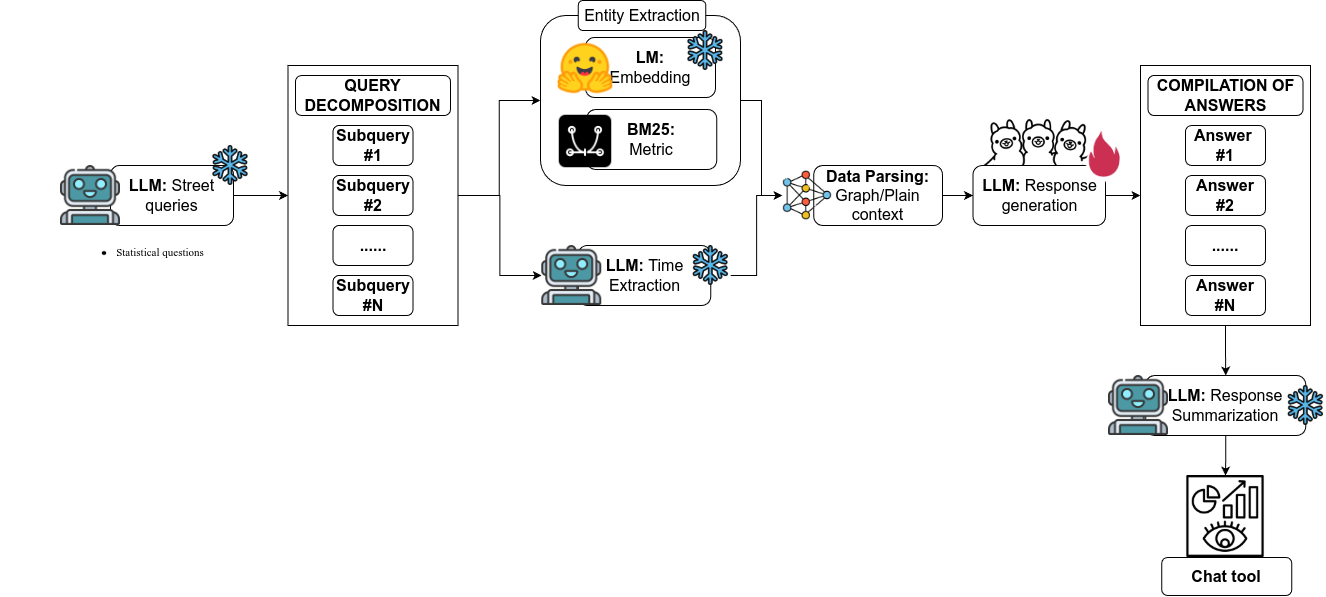
\includegraphics[width=\textwidth]{images/PFC3.drawio.png}
    \caption{Proposed Pipeline - Phase 1}
    \label{fig:proposal_f1}
\end{figure}

\subsection{Phase 2: Expected Next Semester}

\begin{itemize}
    \item \textbf{Synthetic Dataset Generation}: The capabilities of proprietary LLMs will be leveraged to generate synthetic answers (\cite{Nvidia2024KaggleMath}, \cite{Liu2024NLDriven}) based on the formulated questions and the retrieval mechanism. The generated chain-of-thought (CoT) reasoning and associated code will be stored for fine tune the selected LLMs.
    \item \textbf{Model Fine-tuning and Evaluation}: The selected LLMs will be fine-tuned using the expanded dataset, and their performance will be assessed using metrics such as BLEU, ROUGE, BertScore, and METEOR.
\end{itemize}


% \section{Benchmarks}

% \subsection{Estructura de los \textit{datasets}}

% \section{Entrenamiento/Optimización del modelo}

% \section{Evaluación del modelo}

